\noindent
\begin{definition}
Let the gradient of a model output, $f_i$, with respect to an input vector, $x$ be denoted by $g=\nabla f(x)$.  The total gradient is given by 
\begin{equation}
g_t = \sum_{i=1}^D \nabla f(x)_i
\end{equation}
The gradient norm is given by 
\begin{equation}
g_n = \sqrt{\sum_{i=1}^D |\nabla f(x)_i|^2} = ||\nabla f(x)||_2
\end{equation}
\end{definition}

Both of these measures, along with the gradient itself, are shown for our model as well as a small excerpt of one of the text samples in Figure \ref{fig:saliency}.  We see that the three words with the largest total gradients are ``loved'', ``good'', and ``bad'' which are all sentimental.  First, a differentiable function, $f$, can be locally approximated by
\begin{align}
f(w_j) &\approx f(x_i) + (w_j-x_i)^T\nabla f(x_i) \\
     &= f(x_i) + w_j^T\nabla f(x_i) - x_i\nabla f(x_i) \\
     &= f(x_i) + w_j^Tg - x_i^Tg \label{approx}
\end{align}
Here are considering specificially the affect of replacing the $i^{th}$ input word vector, $x_i$ with the $j^{th}$ embedding word vector, $w_j$ while all other input vectors remain constant.

\begin{definition}

With the above defintions of $x_i$, $w_j$, and $\nabla f(x_i)$, let
\begin{align}
X &= 
\begin{bmatrix}
x_1, x_2, \dots, x_N
\end{bmatrix} \in M_{D\times N}(\mathbb{R})\\
W &= 
\begin{bmatrix}
w_1, w_2, \dots, w_V
\end{bmatrix} \in M_{D\times V}(\mathbb{R})\\
G &= 
\begin{bmatrix}
\nabla f(x_1), \nabla f(x_2), \dots, \nabla f(x_N)
\end{bmatrix} \in M_{D\times N}(\mathbb{R})
\end{align}
\noindent
The approximated perturbation, $f(w_j)-f(x_i)$, of replacing the $i^{th}$ input with the $j^{th}$ embedding word vector is given by 
\begin{align}
    D_{i,j} = (G^TW)_{i,j} - (G^TX)_{i,i}
\end{align}
\noindent
$D$ is called the approximate delta matrix.
\end{definition}
\noindent
For a perfectly linear function, $f$, $D_{i,j} = f(w_j) - f(x_i)$.  We found that for small output differences, the approximation worked fairly well in that a lesser approximate delta tended to produce a lesser actual delta, as seen in figure \ref{fig:dvhat}.  However, the approximation failed almost completely for large differences, as illustrated in figure \ref{fig:outliers}.  This is not surprising given that the model is highly non-linear but it confirms that using the gradient alone is not a reliable technique for discovering adversarial derivations.

\begin{figure}
    \centering
    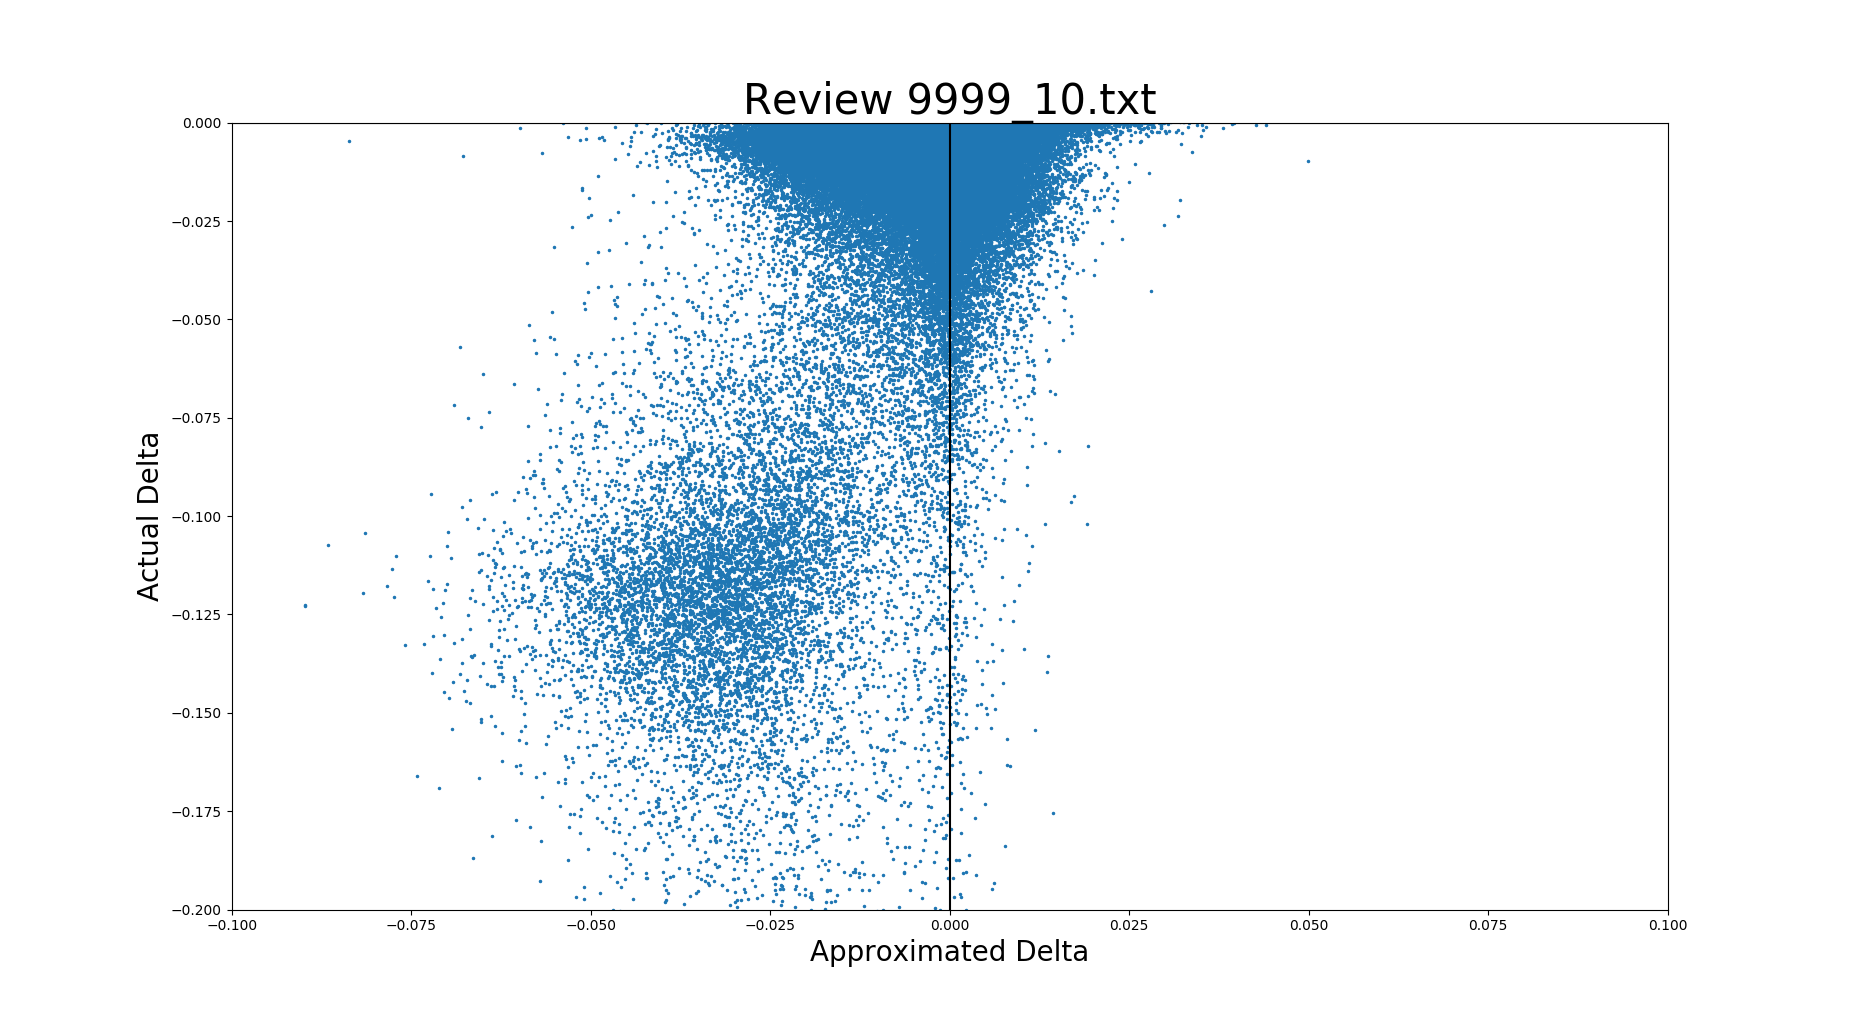
\includegraphics[width=\textwidth]{delta_vs_deltahat.png}
    \caption{Predicted difference in prediction confidence vs. actual difference for sample file 9999\_10.txt}
    \label{fig:dvhat}
\end{figure}

\begin{figure}
\centering
\begin{subfigure}[t]{0.45\textwidth}
  \centering
  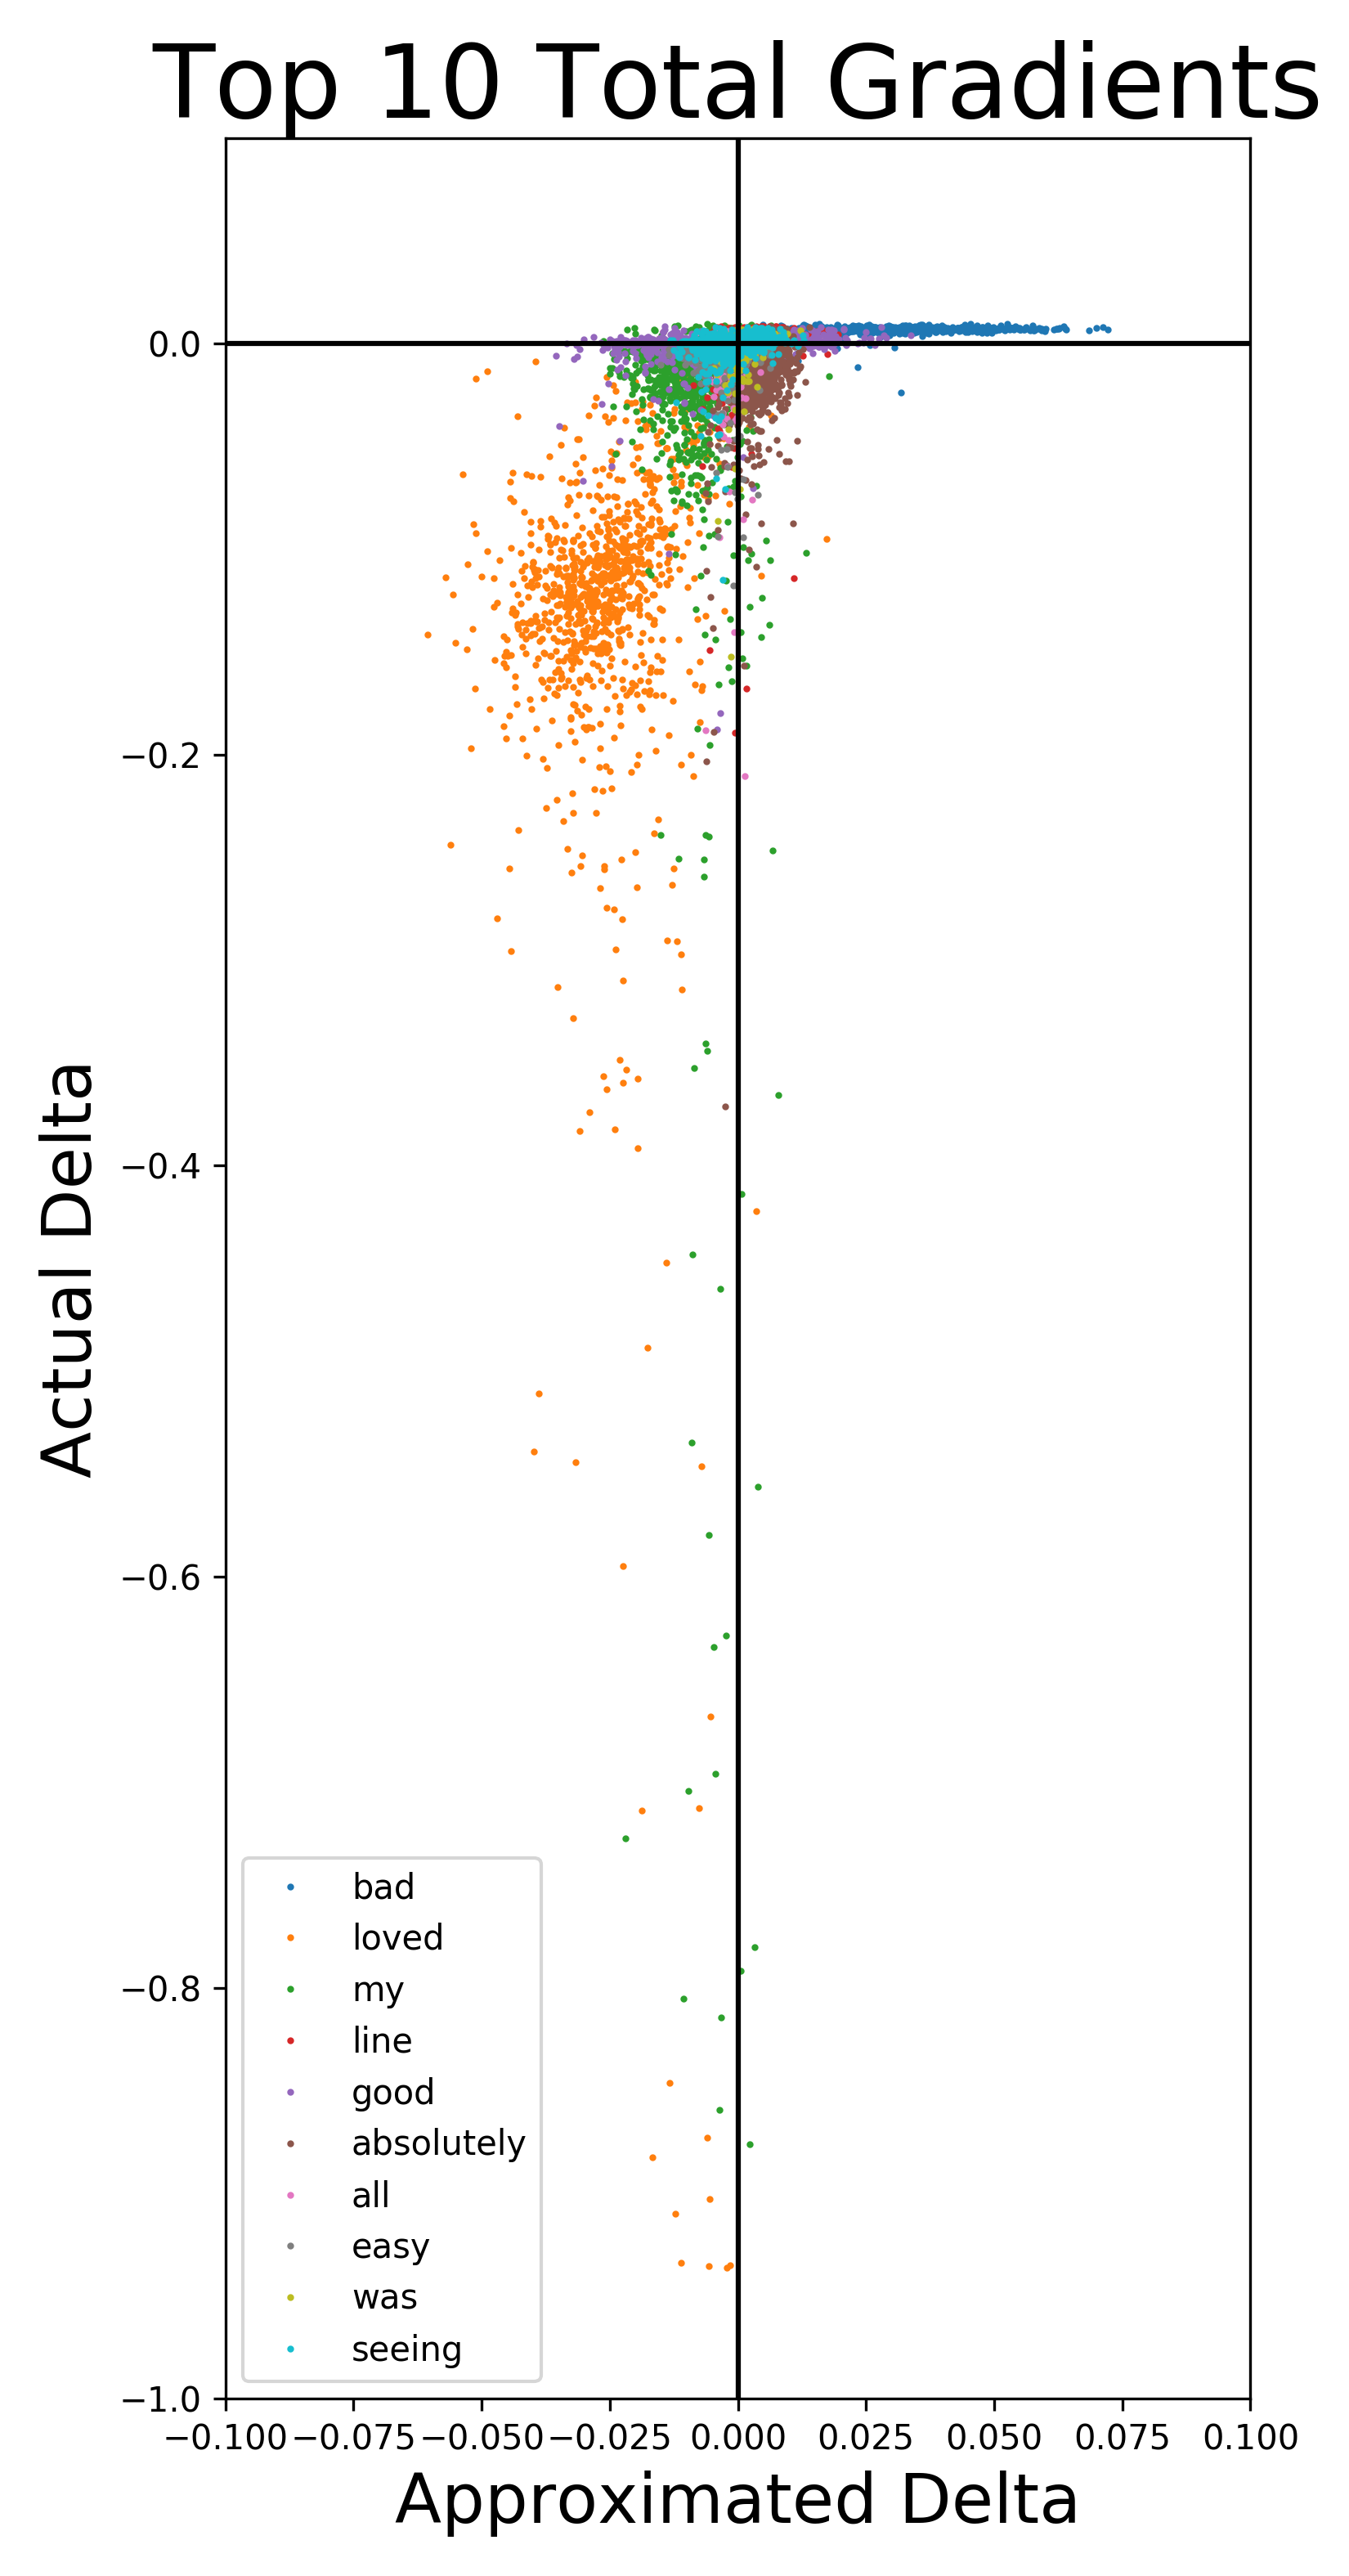
\includegraphics[width=0.9\textwidth]{total_color.png}
  \caption{The words with the top ten largest absolute total gradeints are chosen}
  \label{fig:total_color}
\end{subfigure}\hfill
\begin{subfigure}[t]{0.45\textwidth}
  \centering
  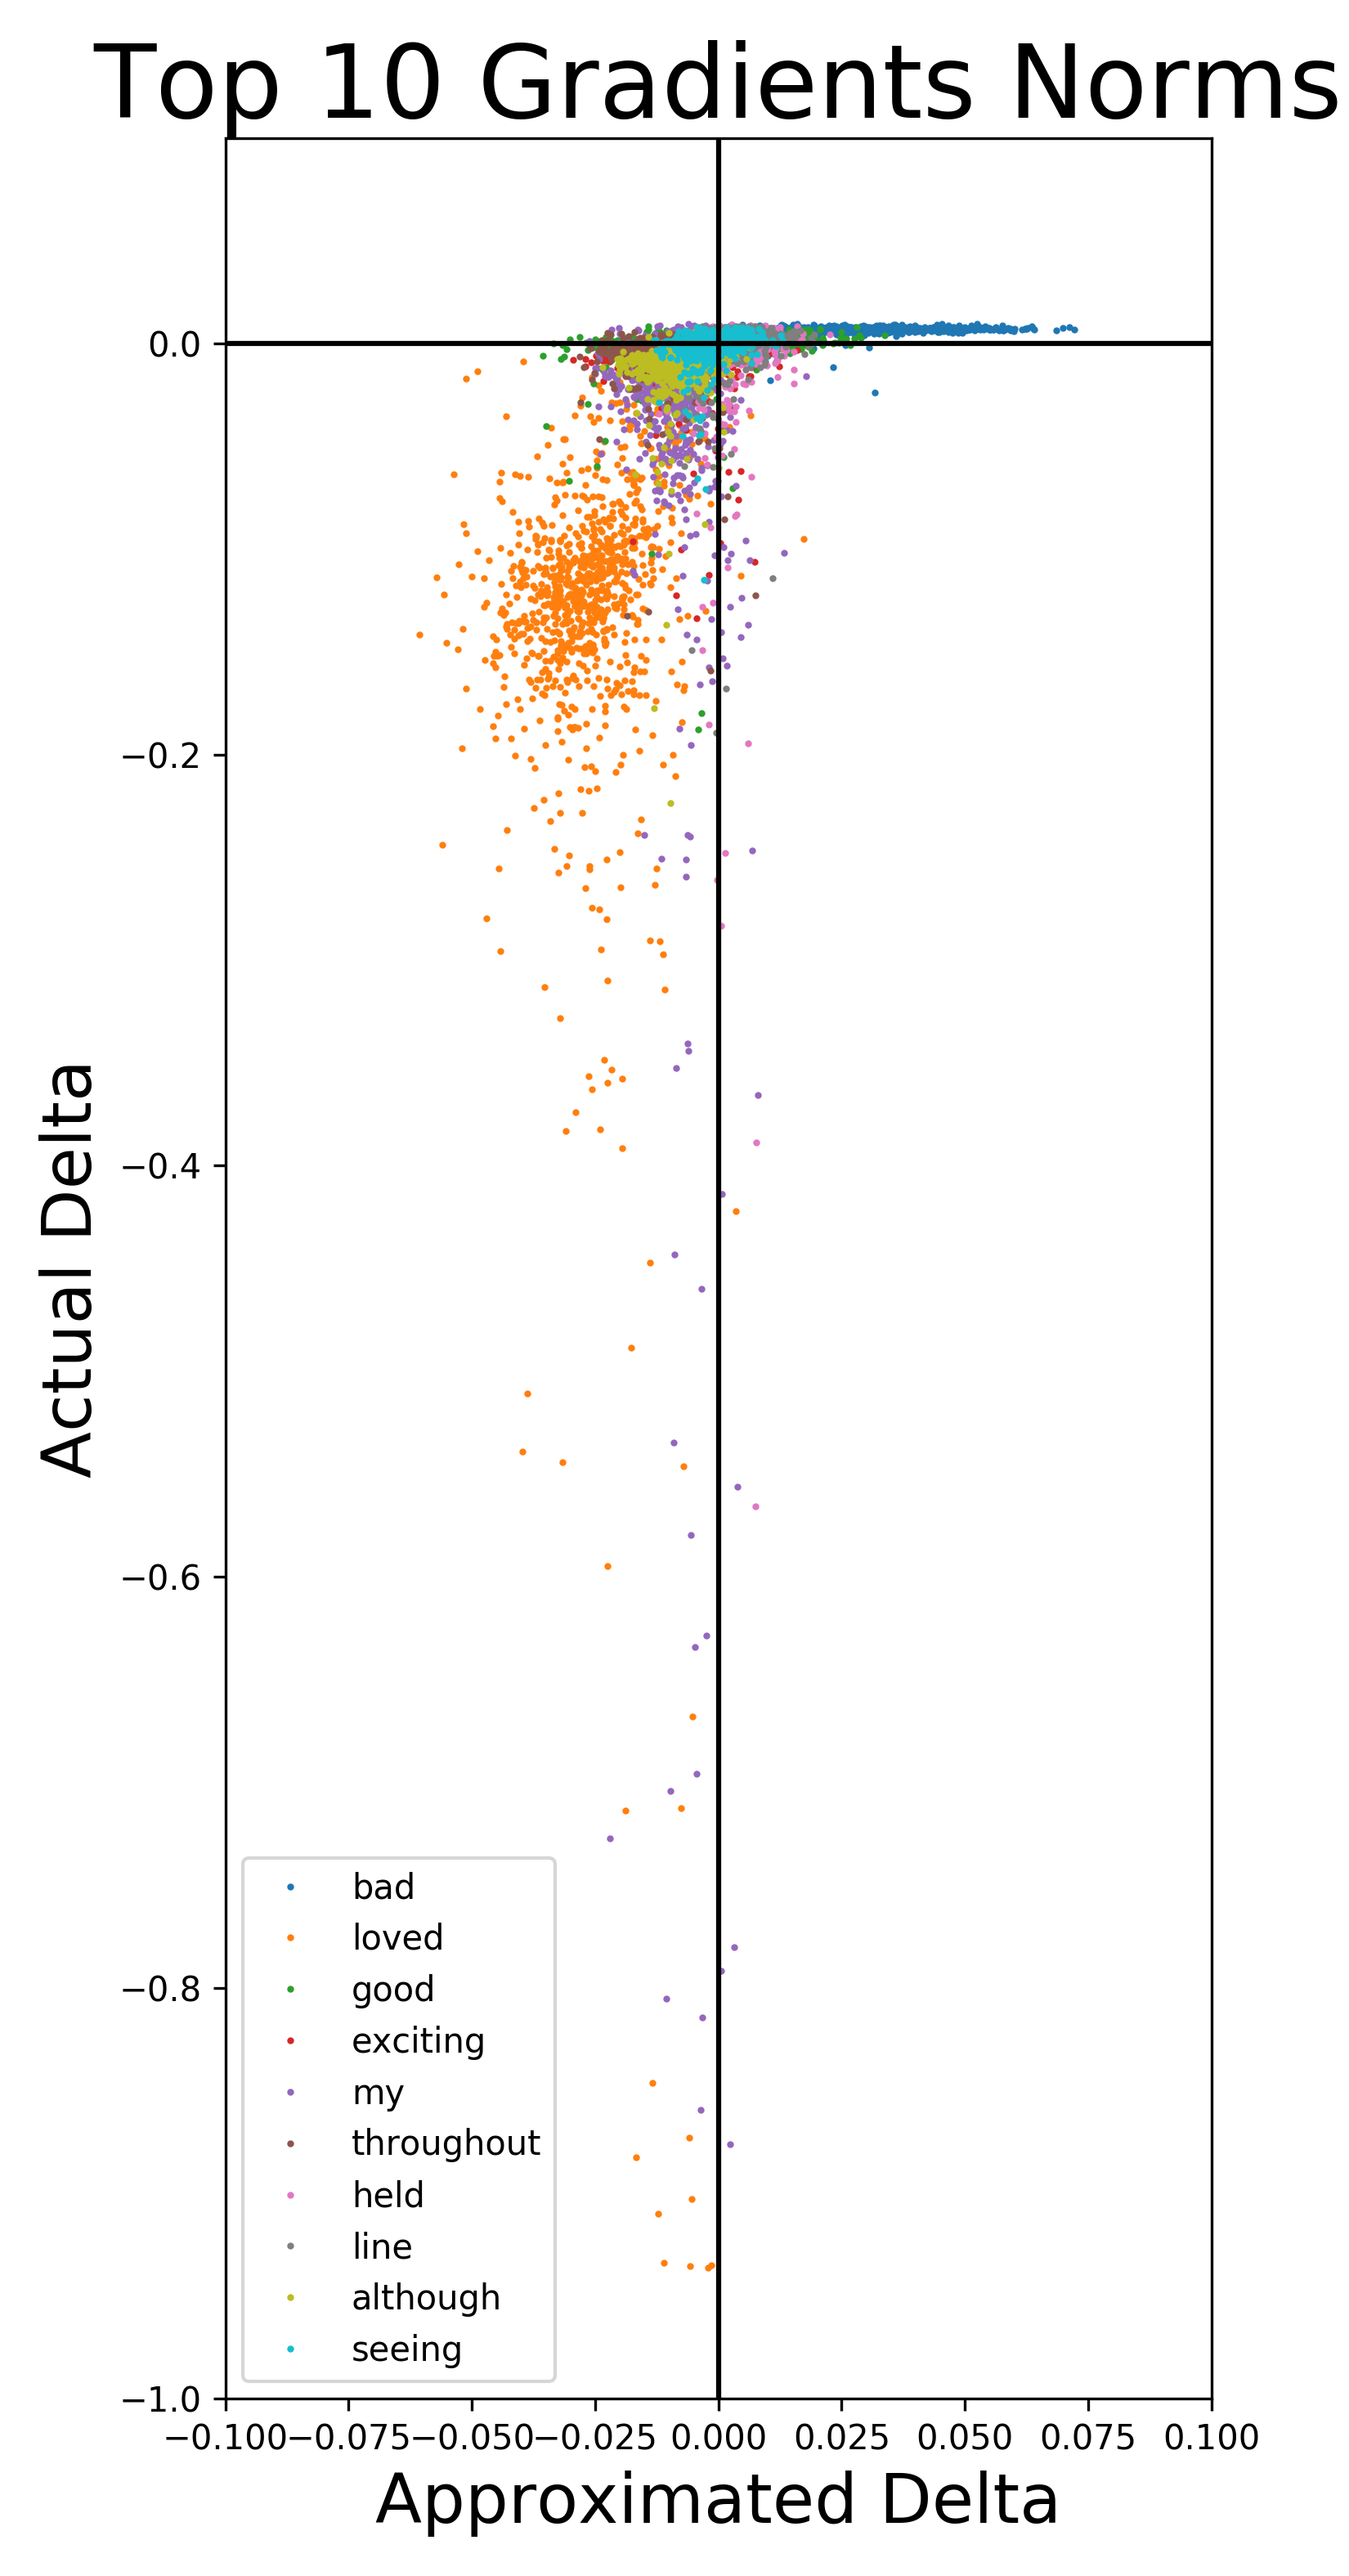
\includegraphics[width=0.9\textwidth]{norm_color.png}
  \caption{The words with the top ten largest gradient norms are chosen}
  \label{fig:norm_color}
\end{subfigure}
\caption{The predicted change in classifier confidence vs. the actual change.  Only the most common 1,000 words are considered in replacement for this example.  The words are listed in the legend in order of decreasing value.}
\label{fig:outliers}
\end{figure}

We see that individual $\hat{D}$ entries are not a good choice for determining which specific words to interchange, but that our measures of gradient may be useful in determining which words are susceptible to attack.  We give motivation with some simplified probabilistic analysis.  Suppose that each of the embedding dimensions is distributed independently and identically across words, with some mean, $\mu$ and variance, $\sigma^2$.  Let $g = \nabla f(x_i)$ for a given word vector, $x_i$ and suppose we replace it with a random word vector, $w_j$.  Recall equation \ref{approx}, we are interested in estimating the term $w_i^Tg = g^Tw_i$ probabilstically since the term $x_i\nabla f(x_i)$ is fixed for a given word.  Let $v=w_i$ and $u=x_i$, then randomly replacing $u$ with another word vector, we have
\begin{equation}
\E{g^Tv} = \E{\sum_{i=1}^D{g_iv_i}} = \sum_{i=1}^D{g_i\E{v_i}} = \mu\sum_{i=1}^D{g_i} = \mu g_t
\end{equation}
\noindent
If we are interested in purposefully altering classification, however, we might be more interested in the expected maximum value of $g^Tv$, that is,
\begin{equation}
Z(g) = \E{\underset{0\leq n\leq V}{\max}\,{g^Tv_n}}
\end{equation}
\noindent
Unfortunately, there is no simple expression which captures this value.  However if we assume that $v_{n,i}$ is distributed normally, we have 
\begin{equation}
Z(g) = \E{\underset{0\leq n\leq V}{\max}\,{g^Tv_n}} = \E{\underset{0\leq n\leq V}{\max}\,{\sum_{i=1}^D{g_i}v_{n,i}}} = \E{\underset{0\leq n\leq V}{\max}\,{p_n}}
\end{equation}
\noindent
where $p_n \sim \mathcal{N}(\mu g_t,\sigma^2 g_n^2)$  There is still no closed form expression for this value, but there is a known \cite{pm07} upper bound:
\begin{align}
Z(g) &\leq \mu g_t + \sigma g_n\sqrt{2\log{V}}\\
\E{\max \hat{D}_{i,*}} &\leq \mu g_t + \sigma g_n\sqrt{2\log{V}} -u^Tg
\end{align}

\noindent
This inequality is intuitively satisfying.  It says that the expected maximum perturbation grows with both the vocabulary size and the norm of the gradient.  The total gradient also plays a role here, increasing or decreasing the expected maximum depending on the sign.  Empirical study of our embedding and classifier show that the term including standard deviation is usually much larger.  It should be noted that the lower bound on the expected minimum, $Y(g)$, is simply given by a sign reversal of the second term:
\begin{align}
Y(g) &\geq \mu g_t - \sigma g_n\sqrt{2\log{V}} \\
\E{\min \hat{D}_{i,*}} &\geq \mu g_t - \sigma g_n\sqrt{2\log{V}} - u^Tg
\end{align}

\begin{figure}
    \centering
    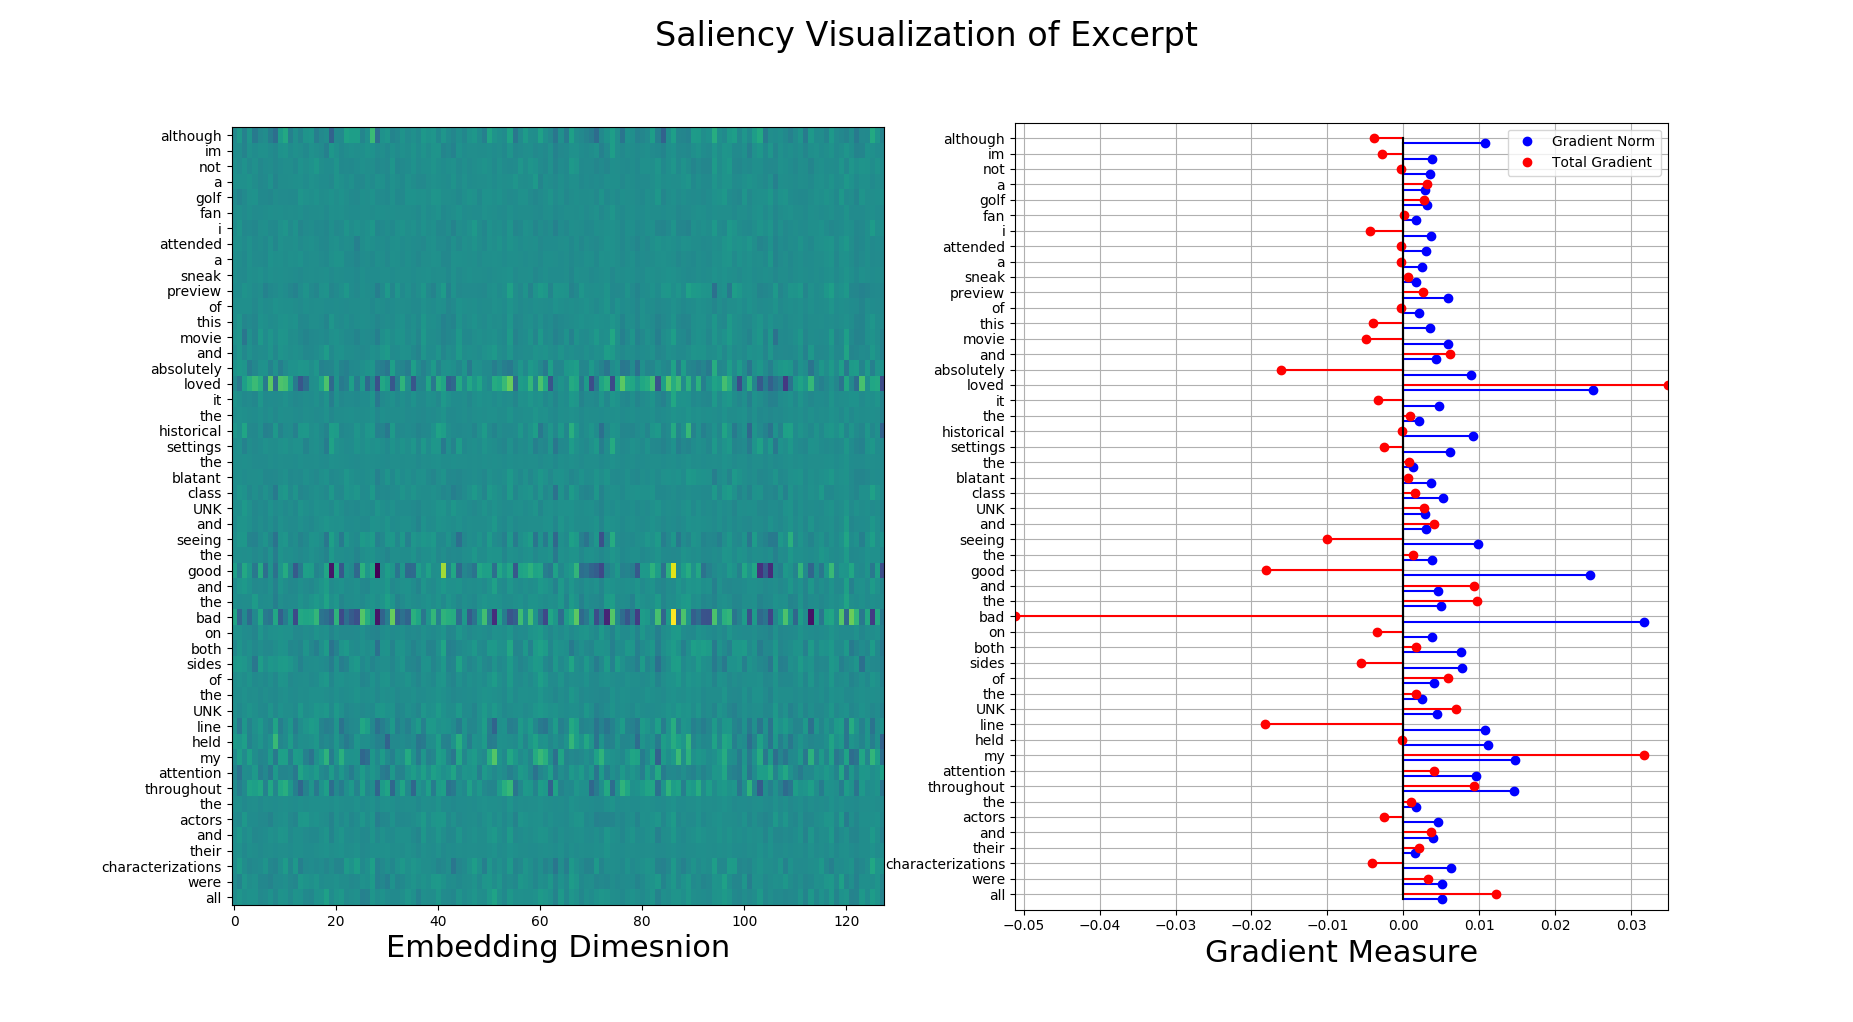
\includegraphics[width=\textwidth]{saliency.png}
    \caption{Different measures of word sentiment/importance}
    \label{fig:saliency}
\end{figure}

In our word embedding, the average value of $\mu$ was $-0.017$, but there was significant variation across embedding dimension.  The average standard deviation was fairly constant over embedding dimension, with a value of $0.55$.  The exact value of the result is not important however.  What this tells us is that words associated with larger gradient norms have a proportionally larger chance of producing an outlier, at least according to the linear approximation.
